\section{Experimentation}
\label{sec:validation}

This experimentation section is comprised of two parts. The first part focuses
on highlighting the behaviour of \NAME{} on extreme cases. The measurements
capture the effect of a large number of insert operations on the identifier
sizes. We synthesized different editing behaviours. Analyses are made step by
step to bring out the contribution of each component to \NAME{}. Previous
experiments~\cite{ahmed2011evaluating,preguica2009commutative,weiss2009logoot}
focused on average setups and did not consider such extreme setups.

The second part of experiments aims to validate if \NAME{} also performs well
on average setups.  In order to do so, we compare Logoot identifiers to \NAME{}
identifiers on representative Wikipedia pages with antagonist editing
behaviours. We choose Logoot as it delivers overall best performances for
variable-size sequence CRDTs according to~\cite{ahmed2011evaluating}.

The experiments focus on the digit part of identifiers. Indeed, the source and
clock part of identifiers are common to all the variable-size identifiers
approaches. They do not impact on the complexity and can be drastically
compressed. Consequently, it is the digit part that reflects the significant
improvements.

To evaluate \NAME{} performance, we developed a Java framework called LSEQ and
released the source on GitHub platform under the terms of the GPL
licence~\footnote{\url{https://github.com/Chat-Wane/LSEQ}}.

\subsection{Synthetic Documents Experiments}
\label{ssec:components}

We designed three experimental setups of synthetic sequences, namely monotone
editing behaviour in one position (first and last position), and totally random
insertions. The monotonic insertions algorithms choose a particular element and
continuously insert new elements before/after this element. For the front
editing, it targets the beginning of the document and inserts
continuously after it. The end editing, it targets the end of the
document and inserts continuously before it. The random behaviour randomly
inserts elements in the range $[0-doc.size[$. The insertions algorithms perform
a large number of insert operations on the sequence (up to
$10^6$). Furthermore, each operation only concerns one element at a time.

In these experiments, we measure the average bit-length of the digit part of
identifiers on four different configurations. In order of appearance: a simple
\emph{boundary+} strategy (\textbf{B}), a base doubling (\textbf{D}) at each
new depth, a Round-Robin strategy choice (\textbf{RR}) and a random strategy
choice with base doubling (\textbf{\NAME}).

\paragraph{Boundary \textbf{B} Experiment}

\begin{figure}
\begin{center}
\small
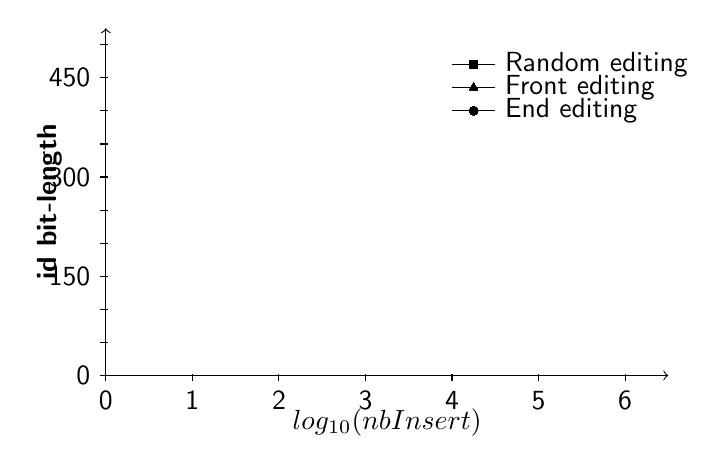
\begin{tikzpicture}[scale=0.7,x=1.57cm, y=0.6cm,font=\sffamily]
%Axis
    \draw[->] (0,0) -- coordinate (x axis mid) (6.5,0);
    \draw[->] (0,0) -- coordinate (y axis mid) (0,10.5);
%Ticks
    	\foreach \x        in { 0,
                              1,
                              2,
                              3,
                              4,
                              5,
                              6}
                              {
     		\draw (\x,1pt) -- (\x,-3pt) node[anchor=north] {\x};}

     	\foreach \y/\ytext in { 0/0,
                              1/,
                              2/,
                              3/150,
                              4/,
                              5/,
                              6/300,
                              7/,
                              8/,
                              9/450,
                              10/} {
     		\draw (1pt,\y) -- (-3pt,\y) node[anchor=east] {\ytext} ;}
%Labels      
	\node[below=0.3cm] at (x axis mid) {$log_{10}(nbInsert)$};
        \node[rotate=90, below=-1.0cm] at (y axis mid) {\textbf{id
            bit-length}};

%Plots
	\draw plot[mark=*, mark options={fill=black}] file
              {weissDataQueue.data}; \draw plot[mark=triangle*, mark
                options={fill=black} ] file {weissDataFront.data}; \draw
              plot[mark=square*, mark options={fill=black}] file
              {weissDataRand.data};

    
	%legend
	\begin{scope}[shift={(4,8)}] 
	\draw (0,0) -- plot[mark=*, mark options={fill=black}] (0.25,0) --
        (0.5,0) node[right]{End editing}; \draw[yshift=\baselineskip] (0,0)
        -- plot[mark=triangle*, mark options={fill=black}] (0.25,0) -- (0.5,0)
        node[right]{Front editing}; \draw[yshift=2*\baselineskip] (0,0) --
        plot[mark=square*, mark options={fill=black}] (0.25,0) -- (0.5,0)
        node[right]{Random editing};
	\end{scope}

\end{tikzpicture}

\caption{Simple \emph{boundary+} setup with $base=2^{10}$ and $boundary=10$}
\label{fig:dimlogexperiment}
\end{center}
\end{figure}

\begin{asparadesc}
\item[Objective:] to show that \emph{boundary+} does not adapt itself neither
  to any monotonic editing behaviour nor to the number of insert
  operations. The expected space complexity is linear compared to the number of
  inserts in any monotonic editing behaviour. The random editing should lead to
  a logarithmic size of identifiers.

\item[Description:] the measurements concern the average bit-length of the
  digit part of identifiers. The checkpoints are 100, 1000, 5000, 10000, 50000,
  100000 insert operations. The experimental setup is \textbf{B} with the
  following parameter values: a \emph{boundary+} strategy with $boundary=10$
  and a constant $base=2^{10}$. It corresponds to the Logoot approach with
  lower values.

\item[Results:] Figure~\ref{fig:dimlogexperiment} shows on the x-axis
  the number of insertions with a logarithmic scale and on y-axis the
  average bit-length of identifiers. As expected the identifiers size
  grows when the number of insertions increases. \textbf{B} handles
  the random editing behaviour with a logarithmic average growth of
  its identifiers. However, with both front and end editing
  behaviour, the curve is linear compared to the number of insertions.
  The end editing remains acceptable in comparison of front editing,
  but the linear growth would eventually lead to the need of a costly
  re-balance protocol.

\item[Reasons:] The front and end editing behaviours tend to unbalance the
  underlying tree model of \textbf{B}. The \emph{boundary+} allocation strategy
  has been designed to handle edition at the end. It reserves more space
  for identifiers at the end, predicting future insertions. The obverse is less
  space for identifiers at front, therefore the front editing behaviour
  unbalances the tree even more quickly (leading to a worst-case space
  complexity of the total identifier size of $O(nb\_insert^2)$). For the same
  reason, the random editing behaviour leads to logarithmic space complexity:
  the tree model is balanced.
\end{asparadesc}

\paragraph{Base doubling \textbf{D} experiment}

\begin{asparadesc}
\item[Objective:] to show that \textbf{D} is not suitable in any case because
  it does not adapt on the editing behaviour.  However, it constitutes an
  improvement over \textbf{B} due to its scalability in terms of insertions
  number.  Indeed, it has a sub-linear upper-bound when the editing behaviour
  is the expected one. Since \textbf{D} uses a \emph{boundary+} allocation
  strategy, the sub-linear upper-bound is on the end editing. On the other
  hand, the expectation on the front editing is even worse than the first
  experiment (with \textbf{B}). The random editing should stay with its
  logarithmic shape unchanged.

\item[Description:] like the previous experiment, this experimentation concerns
  the average bit-length of identifiers. The \textbf{D} setup provides the new
  identifiers.  \emph{boundary+} and base doubling compose this setup. The
  variables are $boundary=10$ and a base starting from $base=2^{4+depth}$. The
  measures are taken at 100, 1000, 5000, 10000, 50000, 100000, 500000
  insertions.

\item[Results:] Figure~\ref{fig:doubleexperiment} shows on the x-axis the
  number of insertions on a logarithmic scale, and on the y-axis the average id
  bit-length. Like \textbf{B}, \textbf{D} provides constantly growing
  identifiers. When the editing behaviour is the expected one, the growth is
  sub-linear compared to the number of insertions. Otherwise, the growth is
  quadratic. Given this, \textbf{D} alone is better than \textbf{B} when the
  current editing behaviour is known. In our context where we have no prior
  knowledge of the editing behaviour, \textbf{D} alone is unsafe.

\item[Reasons:] the base doubling assumes that a high number of insertions
  triggered the creation of previous levels in the tree. Thus, it enlarges the
  number of available identifiers in the new level. If the insertions saturated
  the previous levels, then it verifies this hypothesis, resulting in an
  efficient allocation. Of course, if the base doubling hypothesis is false, in
  the worst case, each new level will contain only one identifier. Each one of
  these identifiers will have a space complexity equal to
  $\sum\limits_{i=1}^{n}{(log_2(b) + i)}$ where $n$ is the number of insertions
  and $b$ is the departure base.
\end{asparadesc}

\begin{figure}
\small
\begin{center}
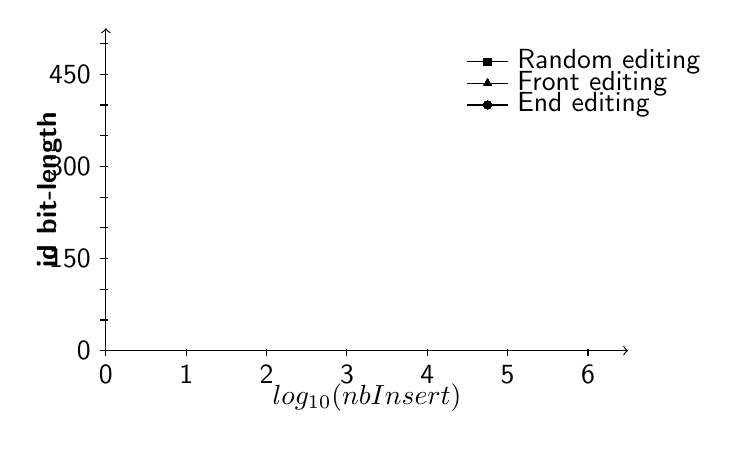
\begin{tikzpicture}[scale=0.65,x=1.57cm,y=0.6cm,font=\sffamily]

%Axis
    \draw[->] (0,0) -- coordinate (x axis mid) (6.5,0);
    \draw[->] (0,0) -- coordinate (y axis mid) (0,10.5);
%Ticks
    	\foreach \x        in { 0,
                              1,
                              2,
                              3,
                              4,
                              5,
                              6}
                              {
     		\draw (\x,1pt) -- (\x,-3pt) node[anchor=north] {\x};}

     	\foreach \y/\ytext in { 0/0,
                              1/,
                              2/,
                              3/150,
                              4/,
                              5/,
                              6/300,
                              7/,
                              8/,
                              9/450,
                              10/} {
     		\draw (1pt,\y) -- (-3pt,\y) node[anchor=east] {\ytext} ;}
%Labels      
	\node[below=0.3cm] at (x axis mid) {$log_{10}(nbInsert)$};
        \node[rotate=90, below=-1.0cm] at (y axis mid) {\textbf{id
            bit-length}};
        
%Plot
  \draw plot[mark=*, mark options={fill=black}]
  file {doubleDataQueue.data};
  \draw plot[mark=triangle*, mark options={fill=black} ] 
  file {doubleDataFront.data};
  \draw plot[mark=square*, mark options={fill=black}] 
  file {doubleDataRand.data};
    
%legend
  \begin{scope}[shift={(4.5,8)}] 
    \draw (0,0) -- 
    plot[mark=*, mark options={fill=black}] (0.25,0) -- (0.5,0) 
    node[right]{End editing};
    \draw[yshift=\baselineskip] (0,0) -- 
    plot[mark=triangle*, mark options={fill=black}] (0.25,0) -- (0.5,0)
    node[right]{Front editing};
    \draw[yshift=2*\baselineskip] (0,0) -- 
    plot[mark=square*, mark options={fill=black}]  (0.25,0) -- (0.5,0)
    node[right]{Random editing};
  \end{scope}
\end{tikzpicture}

\caption{Base doubling setup \textbf{D} ($base=2^{4+id.size}$, $boundary=10$)}
\label{fig:doubleexperiment}
\end{center}
\end{figure}

\paragraph{Round-Robin alternation \textbf{RR} experiment}

\begin{asparadesc}
\item[Objective:] to show that a Round-Robin alternation between
  \emph{boundary+} and \emph{boundary--} provides identifiers with a linear
  upper-bound and consequently does not scale as regards the number of
  insertions.  However, it is an improvement over \textbf{B} and \textbf{D}:
  with no \emph{a priori} knowledge \textbf{RR} avoids the trivial worst case.

\item[Description:] the experiment focuses on the average bit-length of the
  digit part of identifiers. The configuration is a \textbf{RR} setup with two
  allocation strategies \emph{boundary+} and \emph{boundary--}. The parameters
  value are $boundary=10$, and a constant $base=2^{10}$. The measures are taken
  at 100, 1000, 5000, 10000, 50000, 100000 insertions.

\item[Results:] Figure~\ref{fig:roundrobinexperiment} shows on the x-axis on a
  logarithmic scale the number of insertions performed on the sequence. The
  y-axis presents the average bit-length of the digit part of identifiers.
  While on the random editing behaviour, the identifiers size curve stays in a
  logarithmic shape, front and end editing are both in linear shape. These
  observations mean that like \textbf{B}, \textbf{RR} does not adapt to the
  number of insertions, and, on the opposite of \textbf{B} and \textbf{D} it
  avoids the trivial worst case of front edition. Since every collaborative
  editing behaviour is a composition of front, end and/or random edition,
  \textbf{RR} is more predictable. However, \textbf{RR} remains unsafe because
  it does not take into account the large number of monotonic insertions.

\item[Reasons:] compared to \textbf{B}, the average bit-length of identifiers
  grows two times faster in the case of the end editing behaviour. Indeed, the
  \textbf{RR} alternation of strategies avoids the trivial worst case with the
  inappropriate editing behaviour (in front). This improvement comes at a cost:
  half the time \textbf{RR} does not employ the well suited strategy,
  justifying the multiplicative factor of two. The linear space complexity of
  \textbf{RR} stays unchanged compared to \textbf{B}. Consequently, \textbf{RR}
  cannot adapt to high number of insertions. \textbf{RR} does not overwhelm the
  loss of one level by the gain obtained in succeeding levels.
\end{asparadesc}

\begin{figure}
\small
\begin{center}
\begin{figure}
\small
\begin{center}
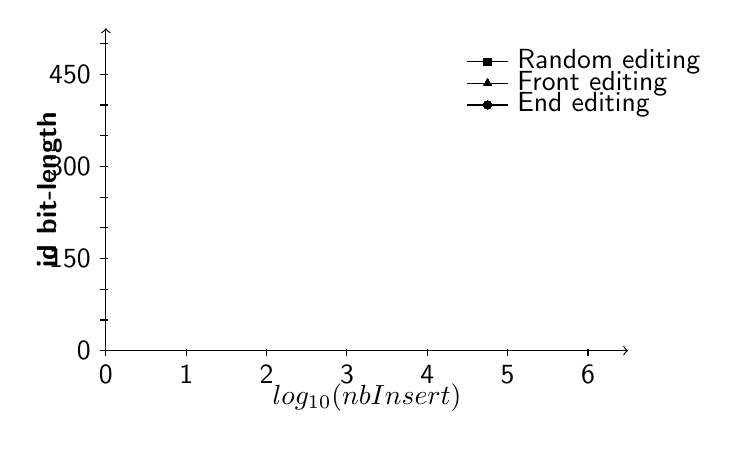
\begin{tikzpicture}[scale=0.65,x=1.57cm,y=0.6cm,font=\sffamily]
%Axis
    \draw[->] (0,0) -- coordinate (x axis mid) (6.5,0);
    \draw[->] (0,0) -- coordinate (y axis mid) (0,10.5);
%Ticks
        \foreach \x in { 0, 1, 2, 3, 4, 5, 6} {
          \draw (\x,1pt) -- (\x,-3pt) node[anchor=north] {\x};}

        \foreach \y/\ytext in { 0/0, 1/, 2/, 3/150, 4/, 5/, 6/300,
          7/, 8/, 9/450, 10/} {
          \draw (1pt,\y) -- (-3pt,\y) node[anchor=east] {\ytext} ;}
%Labels
       \node[below=0.3cm] at (x axis mid) {$log_{10}(nbInsert)$};
       \node[rotate=90, below=-1.0cm] at (y axis mid) {\textbf{id
           bit-length}};

%Plots
        \draw plot[mark=*, mark options={fill=black}] file
              {roundrobinDataQueue.data};
        \draw plot[mark=triangle*, mark
                options={fill=black} ] file {roundrobinDataFront.data};
        \draw plot[mark=square*, mark options={fill=black}] file
              {roundrobinDataRand.data};
%legend
        \begin{scope}[shift={(4.5,8)}]
        \draw (0,0) -- plot[mark=*, mark options={fill=black}] (0.25,0) --
        (0.5,0) node[right]{End editing}; \draw[yshift=\baselineskip] (0,0)
        -- plot[mark=triangle*, mark options={fill=black}] (0.25,0) --
        (0.5,0) node[right]{Front editing}; \draw[yshift=2*\baselineskip]
        (0,0) -- plot[mark=square*, mark options={fill=black}] (0.25,0) --
        (0.5,0) node[right]{Random editing};
        \end{scope}
\end{tikzpicture}
\caption{Round-Robin (\textbf{RR}) alternation of strategies \emph{boundary+}
  and \emph{boundary--} ($base=2^{10}$; $boundary=10$)}
\label{fig:roundrobinexperiment}
\end{center}
\end{figure}

\caption{Round-Robin (\textbf{RR}) alternation of strategies \emph{boundary+}
  and \emph{boundary--} ($base=2^{10}$; $boundary=10$)}
\label{fig:roundrobinexperiment}
\end{center}
\end{figure}


\paragraph{\textbf{\NAME{}} experiment}

\begin{asparadesc}
\item[Objective:] to show that \NAME{} remedies both problems of
  \begin{inparaenum}[(i)]
  \item editing behaviour dependence and
  \item the non-adaptive behaviour as regards the number of insert operations.
  \end{inparaenum}
  The expected space complexity of the identifiers is sub-linear compared to
  the number of insertions, both in front and end editing. The random editing
  stays with the logarithmic behaviour.

\item[Description:] we measure the bit-length of the digit part of
  identifiers. The \NAME{} approach provides the identifiers. It lazily and
  randomly assigns either \emph{boundary+} or \emph{boundary--} to each
  depth. The $boundary$ parameter is set to $10$ and the base is doubled over
  depths. Its departure value is $base=2^{4}$. The checkpoints of measurement
  are 100, 1000, 5000, 10000, 50000, 100000, 500000, 1000000 insertions.
  
\item[Results:] Figure~\ref{fig:lseqexperiment} shows the average bit-length of
  \textbf{\NAME{}} identifiers on the y-axis. The x-axis represents the number
  of insertions on a logarithmic scale. Both front and end editing are now
  sub-linear compared to the number of inserts. On this setup, the curves are
  poly-logarithmic. The average values are close of the \textbf{D} setup. It
  means that \NAME{} loses some depths, but future insertions quickly amortize
  them. More precisely, it means that the base doubling is profitable enough to
  compensate the previous lost depths. These two changes make \NAME{} a
  suitable safe allocation strategy for sequences.

\item[Reasons:] base doubling \textbf{B} performs well if its hypothesis is
  true, i.e., a high number of insertion triggered the creation of levels. The
  random choices of strategy among \emph{boundary+} and \emph{boundary--} makes
  the base doubling hypothesis true with a probability of $1 \over{2}$. So
  eventually, \textbf{\NAME{}} will obtain the expected gain of base
  doubling. This gain is high enough to overwhelm the loss of previous
  levels. It results in a sub-linear upper-bound on the space complexity of
  \textbf{\NAME{}}.
\end{asparadesc}

\begin{figure}
\small
\begin{center}
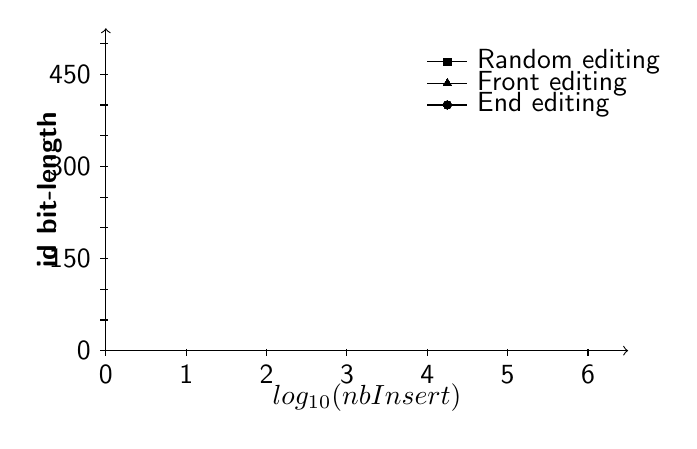
\begin{tikzpicture}[scale=0.65,x=1.57cm, y=0.6cm,font=\sffamily]

%Axis
    \draw[->] (0,0) -- coordinate (x axis mid) (6.5,0);
    \draw[->] (0,0) -- coordinate (y axis mid) (0,10.5);
%Ticks
        \foreach \x in { 0, 1, 2, 3, 4, 5, 6} { \draw (\x,1pt) -- (\x,-3pt)
          node[anchor=north] {\x};}

        \foreach \y/\ytext in { 0/0, 1/, 2/, 3/150, 4/, 5/, 6/300, 7/, 8/,
          9/450, 10/} { \draw (1pt,\y) -- (-3pt,\y) node[anchor=east] {\ytext}
          ;}
%Labels
        \node[below=0.3cm] at (x axis mid) {$log_{10}(nbInsert)$};
        \node[rotate=90, below=-1.0cm] at (y axis mid) {\textbf{id
            bit-length}};

%Plots
        \draw plot[mark=*, mark options={fill=black}] file
              {doublerandomDataQueue.data}; \draw plot[mark=triangle*, mark
                options={fill=black} ] file {doublerandomDataFront.data}; \draw
              plot[mark=square*, mark options={fill=black}] file
              {doublerandomDataRand.data};

%legend
        \begin{scope}[shift={(4,8)}]
        \draw (0,0) -- plot[mark=*, mark options={fill=black}] (0.25,0) --
        (0.5,0) node[right]{End editing}; \draw[yshift=\baselineskip] (0,0)
        -- plot[mark=triangle*, mark options={fill=black}] (0.25,0) --
        (0.5,0) node[right]{Front editing}; \draw[yshift=2*\baselineskip]
        (0,0) -- plot[mark=square*, mark options={fill=black}] (0.25,0) --
        (0.5,0) node[right]{Random editing};
        \end{scope}
\end{tikzpicture}


\caption{Round-Robin (\textbf{RR}) alternation of strategies \emph{boundary+}
  and \emph{boundary--} ($base=2^{10}$; $boundary=10$)}
\label{fig:roundrobinexperiment}
\end{center}
\end{figure}

\subsection{Real Documents Experiments}

In previous section, we demonstrate experimentally a sub-linear upper-bound for
\NAME{}. Next, we aim to confirm the \NAME{} properties on real documents. As
Logoot delivers best overall performances according
to~\cite{ahmed2011evaluating}, we compare \NAME{} with Logoot on Wikipedia
documents as previously done in~\cite{DBLP:journals/tpds/WeissUM10}.

We select Wikipedia documents with a large amount of lines, with front editing
and end editing spectrums. We compare the following two setups:
\begin{inparaenum}[(1)]
  \item Logoot (\textbf{L}) as~\cite{weiss2009logoot} originally described it,
  \item a composition of base doubling and Round-Robin strategy choice
    (i.e. equivalent to \NAME{}) (\textbf{\NAME{}}$^\approx$).
\end{inparaenum}

\paragraph{End Editing in Wikipedia}
\begin{asparadesc}
  
\item[Objective:] to confirm that \textbf{\NAME{}}$^\approx$ and transitively
  \NAME{} brings an improvement on the allocation of identifiers, even in cases
  where previous approaches are known to be good.

\item[Description:] the Wikipedia page
  chosen\footnote{\url{http://fr.wikipedia.org/wiki/Liste_des_bureaux_de_poste_français_classés_par_oblitération_Petits_Chiffres}}
  to run experiments contains a high amount of lines, mainly added at the
  end. The nature of stored data explains the editing behaviour: a list of
  postal marking ids applied to letters. Experiments concern two
  configurations.
  \begin{inparaenum}[(1)]
  \item \textbf{L} with a single \emph{boundary+} strategy, and parameters set
    to $base=2^{64}$ and $boundary=1M$,
  \item \textbf{\NAME{}}$^\approx$ that alternates the two allocation
    strategies \emph{boundary+} and \emph{boundary--}, and parameters set to
    $base=2^{4+depth}$, $boundary=10$.
  \end{inparaenum}

\item[Results:] Figure~\ref{im:poste} shows that, on this document, the
  bit-length of \textbf{\NAME{}}$^\approx$ identifiers is lower than the ones
  of \textbf{L} in the whole document. Table~\ref{tab:queuePage} reflects these
  results: the average bit-length of \textbf{\NAME{}}$^\approx$ identifiers is
  $2.7$ times lower than \textbf{L} identifiers in spite of the fact that the
  average size of \textbf{\NAME{}}$^\approx$ identifiers (i.e. number of
  depths) is $2.36$ times higher. Therefore, \textbf{\NAME{}}$^\approx$ seems
  to be better suited than Logoot on documents with end editing. It
  corroborates the observations made in section~\ref{ssec:components}.

\item[Reasons:] when \textbf{L} has to increase the depth of its identifiers,
  it allocates a large additionnal space. Each new depth costs 64 bits. It
  supposely handles $2^64$ more elements. However, the adding of depth happens
  very quickly when the editing behaviour is not exactly as expected. In
  particular, the spectrum of the document shows very erratic insertions at the
  end (in the references and external links part). On the other hand,
  \textbf{\NAME{}}$^\approx$ tries to allocate ``when it is needed''. It
  explains why minor editing behaviour changes do not affect a lot the
  identifiers size. Furthermore, the base doubling of
  \textbf{\NAME{}}$^\approx$ adapts progressively the allocations to the high
  number of insertions.
\end{asparadesc}
 
\begin{table}[h]
\addtolength{\belowcaptionskip}{-15pt}
  \begin{center}
    \begin{tabular}{|c|c|r|r|}
      \cline{3-4}
      \multicolumn{2}{c|}{} &\textbf{L} &\textbf{\NAME{}}$^\approx$\\
      \cline{3-4}
      \hline
      \multirow{2}{*}{id-length} & avg & $2.65$ & $6.25$ \\
      \cline{2-4}
      &  max & $4$ & $12$ \\
      \hline
      \hline
      \multirow{2}{*}{id-bit-length} & avg & $169.7$ & $61.24$\\
      \cline{2-4}
      & max & $256$ & $150$ \\
      \hline
    \end{tabular}
    \caption{Numerical values of experiments on the Wikipedia page edited at
      the end (corresponding to Figure~\ref{im:poste}).}
    \label{tab:queuePage}
  \end{center}
\end{table}


\begin{figure*}
\addtolength{\belowcaptionskip}{-5pt}
\begin{subfigure}[l]{0.47\textwidth}
  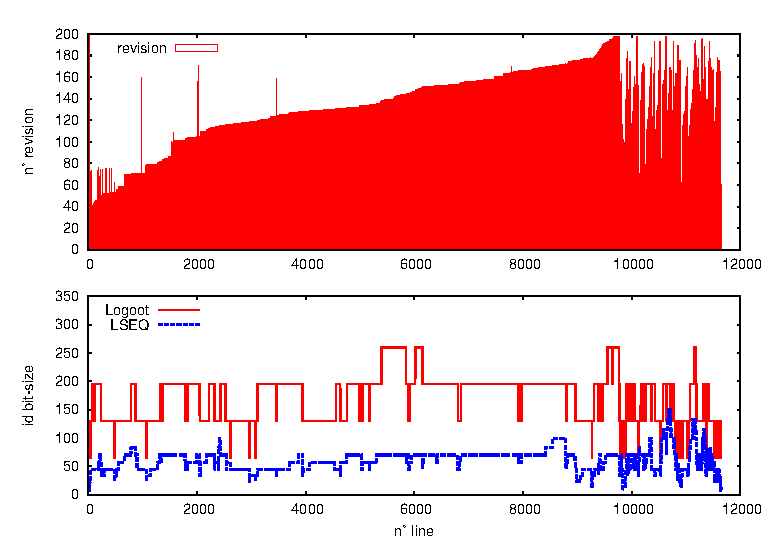
\includegraphics[width=\textwidth]{img/poste.eps}
  \caption{The Wikipedia page has 12k lines and is mostly edited at the
    end. The average bit-lengths of identifiers are $168.7$ and $61.24$ for
    \textbf{L} and \textbf{\NAME{}}$^\approx$ respectively.}
  \label{im:poste}
\end{subfigure}
\hfill
\begin{subfigure}[r]{0.47\textwidth}
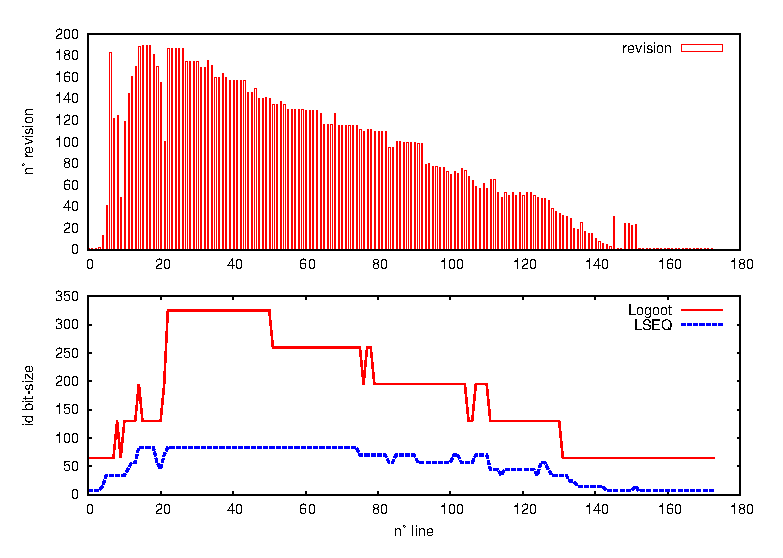
\includegraphics[width=\textwidth]{img/didyouknow.eps}
\caption{The Wikipedia page has 170 lines and is mostly edited at the
  beginning. The average bit-lengths of identifiers are $172.25$ and $51.99$
  $bit/id$ for  \textbf{L} and \textbf{\NAME{}$^\approx$} respectively.}
\label{im:didyouknow}
\end{subfigure}
\caption{The top spectrums reflect the editing behaviour performed on Wikipedia
  pages. The bottom figures shows the identifier bit-length assigned to each
  line. Two configurations: Logoot (\textbf{L}) and Round-Robin with base
  doubling (\textbf{\NAME{}}$^\approx$).}
\end{figure*}

\paragraph{Front Editing in Wikipedia}
\begin{asparadesc}
  
\item[Objective:] to highlight the importance of alternating the allocation
  strategies in \textbf{\NAME{}}$^\approx$. In other words, the
  \emph{boundary+} strategy of \textbf{L} is not sufficient to provide a safe
  allocation system. Finally, to show that \textbf{\NAME{}}$^\approx$
  outperforms \textbf{L} on documents edited at the beginning.

\item[Description:] we choose the Wikipedia
  page~\footnote{\url{http://en.wikipedia.org/wiki/Template_talk:Did_you_know}}. Since
  it is a ``talk'' page, it provides a discussion space. The users mostly
  inserted elements at the beginning of the document. Once again, we make the
  measurements on two configurations.
  \begin{inparaenum}[(1)]
    \item \textbf{L} with a single \emph{boundary+} strategy, and parameters
      set to $base=2^{64}$ and $boundary=1M$,
    \item \textbf{\NAME{}}$^\approx$ with the two allocation strategies
      \emph{boundary+} and \emph{boundary--}, and $base=2^{4+depth}$,
      $boundary=10$.
  \end{inparaenum}

\item[Result:] unsurprisingly, the figure~\ref{im:didyouknow} shows that using
  \textbf{L}, the identifiers bit-length increases very fast in the beginning
  of the document while it quickly stabilizes when \textbf{\NAME{}}$^\approx$
  is used. In Table~\ref{tab:didyouknow}, we observe that the average
  identifiers bit-length of \textbf{\NAME{}}$^\approx$ is $3.31$ times lower
  than the one of \textbf{L}.  The alternation of strategies allows
  \textbf{\NAME{}}$^\approx$ to quickly find a depth where allocation of
  identifiers will be efficient, and thereby to amortize previous depths where
  some spaces could have been wasted.  These observations confirm the results
  of section~\ref{ssec:components}.
  
  \item[Reasons:] \textbf{\NAME{}}$^\approx$ does not favor any editing
    behaviour thanks to its allocation strategies. On the opposite, \textbf{L}
    uses an allocation strategy designed to support end editing, thus, when
    the antagonist behaviour arises, the identifiers size grow very fast.
\end{asparadesc}

\begin{table}[h]
\addtolength{\belowcaptionskip}{-15pt}
  \begin{center}
    \begin{tabular}{|c|c|r|r|}
      \cline{3-4}
      \multicolumn{2}{c|}{} &\textbf{L} &\textbf{\NAME{}}$^\approx$\\
      \cline{3-4}
      \hline
      \multirow{2}{*}{id-length} & avg & $2.69$ & $5.29$ \\
      \cline{2-4}
     &  max & $5$ & $8$ \\
      \hline
      \hline
      \multirow{2}{*}{id-bit-length} & avg & $172.25$ & $51.99$\\
      \cline{2-4}
      & max & $320$ & $84$ \\
      \hline
    \end{tabular}
    \caption{Numerical values of experiments on the Wikipedia page edited at
      the beginning (corresponding to Figure~\ref{im:didyouknow}).}
    \label{tab:didyouknow}
  \end{center}
\end{table}

\subsection{Synthesis}

Experiments evaluated the contribution of each part of \NAME{} allocation
function. They demonstrated that each isolated component cannot achieve
sub-linear space complexity. However, their composition with random choice
among \emph{boundary+} and \emph{boundary--} and a base doubling can achieve
sub-linear space complexity in extreme setups. We also observe this gain on
real documents. Consequently, \NAME{} is suitable for building distributed
collaborative editors that deliver better performance and in a larger scope of
usage than state of art.

